\chapter{A Brief Review of Scattering Functions}
\label{chapter:appearance}

In this chapter we will review a hierarchy of scattering functions. 
Scattering functions describe how incoming and outgoing directions of the light are related for a surface at which light-material interaction occurs \cite{dong}.
Such functions are possible to measure for a given object.
After obtaining the data, scattering functions can provide all the necessary information to render the material appearance. 
Due to diversity of material properties, different functions were introduced.  
In order to chose suitable scattering function for capturing certain scattering effects for a particular type of material,
it is important to be aware of the hierarchy of scattering functions.

	
\section{Light-Material Interaction}
\label{section:light}	
Before defining any scattering functions of light the basics light-material interaction.
Generally speaking, when light hits a material's surface, a sophisticated light-matter process happens.
Such process depends on physical properties of the material as well as on physical properties of light\cite{wynn}. 
For instance, an opaque surface such as wool will reflect light differently than a smooth surface with high specularities such as metal. 

 When light makes a contact with a material, three types of interactions may occur: light \emph{reflection}, light \emph{absorption} and light \emph{transmittance}. 
 Light \emph{reflection} is the change in direction of light at an interface between two different media so that light returns into the medium from which it originated.
 Light \emph{absorption} is a process when a light is being taken up by a material and transformed into internal energy of the material, for instance thermal energy.
 When a material is transparent, light \emph{transmittance} can occur.
 It means, that the light travels through the material and exits on the opposite side of the object. 
   Figure \ref{fig:light_example} demonstrates these 3 types of interactions.
  
 Because light is a form of energy, conservation of energy says that \cite{wynn}
 \begin{center} 
\emph{incident light at a surface = light reflected + light absorbed + light transmitted}
 \end{center}
 


\section{General Scattering Function}
\label{section:grf}
 
To define the general scattering function(GSF) imagine the light-wave hitting the surface at time $t_{i}$ and position $x_{i}$ and with wavelength $\lambda_{i}$\cite{star2004}.
 With a given local coordinate system at a surface point, the incoming direction of light can be defined as $(\theta_{i} ,\phi_{i})$.
 Light travels inside the material and exits the surface at position $x_{o}$ and time $t_{o}$, with possibly changed wavelength $\lambda_{o}$ in the outgoing direction $(\theta_{o} ,\phi_{o})$.
 Figure  \ref{fig:light_example} illustrates the process.
 
 
  \begin{figure}[h]
 \centering
 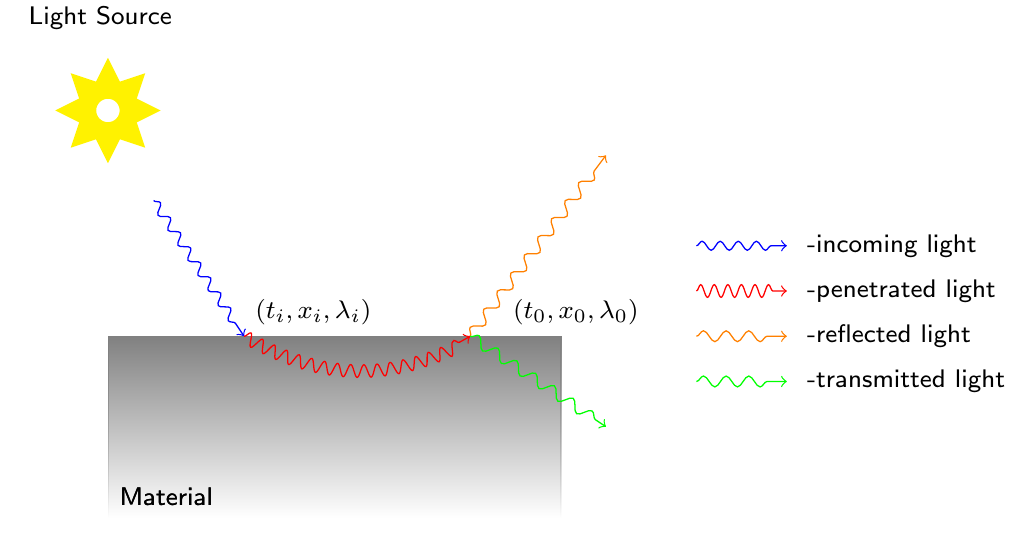
\includegraphics[width=1.0\textwidth]{figures/light}
 \caption[Example of Light-Material interaction] {
 	{\bf Example of Light-Material interaction.}

 }
 \label{fig:light_example}
\end{figure}
According to the description we get a GSF
 \begin{center} 
 
$GSF(t_{i},t_{o},x_{i},x_{0,}\theta_{i} ,\phi_{i},\theta_{o},\phi_{o},\lambda_{i},\lambda_{o})$
 \end{center}
in which  spatial positions $x_{i,o}$ are 2-D variables.
This function describes light interaction for each surface point for any incoming light and outgoing direction at certain time.
Such function compromise 12 parameters. Also, note that we neglected light transmittance, which would even further complicate the function.




\section{Bidirectional Scattering-Surface Reflectance Distribution Function}
\label{section:BSSRDF}
 Since the measurement, modeling and rendering of a 12-D GSF function is currently not practical, additional assumptions have to be made to simplify the function.
 Usually such assumption are made \cite{star2004}:

\begin{itemize}
 \item light interaction takes zero time ($t_{i}$  = $t_{o}$)
 \item wavelength is separated into the three color bands red, green and blue ($\lambda_{r,g,b}$)
 \item interaction does not change wavelength ($\lambda_{i}= \lambda_{0}$)
\end{itemize}

After mentioned assumptions we get a 8-D bidirectional scattering-surface reflectance distribution function (BSSRDF)
 \begin{center}
$BSSRDF(x_{i},x_{o}\theta_{i} ,\phi_{i}\theta_{o} ,\phi_{o})$
 \end{center}


BSSRDF describes various light interactions for heterogeneous both translucent and opaque materials.
That is why BSSRDF can be used for rendering materials such as skin, marble, milk and other objects which do not look realistic without subsurface scattering. 
Subsurface scattering is a process when light penetrates an object at an incident point, travels inside the object and exists at a different point of the object.

\section{Bidirectional Texture Function}
\label{section:btf}
If we simplify further and assume that

\begin{itemize}
 \item light entering a material exits at the same point $x_{i}=x_{o}$, while internal subsurface scattering is still present
\end{itemize}

we will get a 6-D bidirectional texture function (BTF).

Subsurface scattering, self-occlusion, self-shadowing  are still present, now it just comes pre-integrated, i.e. it can be defined through BSSRDF \cite{star2004}:
 \begin{center}
$ BTF(x,\theta_{i} ,\phi_{i},\theta_{o} ,\phi_{o})=\int_{S}BSSRDF(x_{i},x,\theta_{i} ,\phi_{i},\theta_{o} ,\phi_{o}) dx_{i}$
 \end{center}
  The assumption that $x_{i}=x_{o}$ simplifies measuring, modeling and rendering of the scattering function. 
 As we can see the BTF integrates subsurface scattering from neighbouring surface locations. 

\section{Bidirectional Subsurface Scattering Distribution Function}
\label{section:BSSDF}

Another possible reduction of the 8-D BSSRDF is to assume that we deal with a homogeneous surface \cite{dong}, i.e.
\begin{itemize}
 \item subsurface scattering depends only on relative surface positions of incoming and outgoing light $(x_{i}-x_{o})$
\end{itemize}
  Simply saying it means that scattering do not vary over a surface.
 With such assumption we get a 6D function that known as a bidirectional subsurface scattering
distribution function (BSSDF).
 \begin{center}
$BSSDF(x_{i}-x_{o},\theta_{i} ,\phi_{i},\theta_{o} ,\phi_{o})$
 \end{center}
 BSSDF represents homogeneous materials for which subsurface scattering is a significant feature of their overall appearance.
 For instance, BSSDF accounts for objects such as water, milk, human skin, and marble.

\section{Bidirectional Reflectance Distribution Function}
\label{section:brdf}

If we assume the following for a BSSDF that

\begin{itemize}
 \item there is no spatial variation 
 \item no self-shadowing
 \item no self-occlusion
 \item no inter-reflections
 \item no subsurface scattering
 \item energy conservation
 \item reciprocity  $BRDF(\theta_{i} ,\phi_{i},\theta_{o} ,\phi_{o})$=$BRDF(\theta_{o} ,\phi_{o},\theta_{i} ,\phi_{i})$.
\end{itemize}

 we get a 4-D bidirectional reflectance distribution function (BRDF)
 \begin{center}
$BRDF(\theta_{i} ,\phi_{i},\theta_{o} ,\phi_{o})$.
 \end{center}
Nicodemus et al. \cite{Nicodemus} was the one who proposed the BRDF. 
Two principal properties of the BRDF were introduced, i.e. \emph{energy conservation} and \emph{reciprocity}. 
\emph{Energy conservation} law states that the total amount of outgoing light from a surface cannot exceed the
original amount of light that arrives at the surface \cite{wynn}. 
 \emph{Reciprocity} says that if we swap incoming and outgoing directions BRDF stays the same.
If either of these conditions are not satisfied then such BRDF is called \emph{apparent} BRDF (ABRDF) \cite{abrdf}.

It is quite difficult to create a mathematical model for a BRDF that satisfies reciprocity,
energy conservation and the same time produces realistic images. However, most BRDF's models do not satisfy these conditions and still get plausible rendering results.
For instance, Phong model is the most well-known shading model in computer graphics. 
The traditional Phong model satisfy neither energy conservation nor reciprocity, but can still render many materials realistically plausible.
Usually, such materials are of opaque and flat nature, for example plastic materials.
The Phong model is an empirical model and is designed to fit the original function, often based on simple formulas which were derived from observations.


\section{Spatially Varying Bidirectional Reflectance Distribution Function}
\label{section:svbrdf}
If spatial dependence for BRDF takes place, we get a 6-D spatially varying BRDF (SVBRDF)


 \begin{center}
$SVBRDF(x,\theta_{i} ,\phi_{i},\theta_{o} ,\phi_{o})$.
 \end{center}
 Assumptions are the same as for the BRDF, except now spatial dependence is present.
 
A SVBRDF is closely related to a BTF. The SVBRDF and the BTF almost the same scattering function, the difference is in scattering process. 
Changes in scattering at local position $x$ for the BTF are influenced from neighbouring 3D surface geometry, as a result the self-shadowing, masking and inter-reflections are captured by the BTF.
On the other side, the spatial dependence of a SVBRDF describes variations in the optical properties of a surface \cite{haindl_visual}.


 
A SVBRDF represents structures at micro-scale level, which corresponds to near flat opaque materials. On the other side, a BTF capture structure both at macro and micro scales.
 That means that the BTF takes into account influences from local neighbourhood structures. Even though measurement, compression, rendering are more efficient for the SVBRDF, 
 the BTF can produce better visual results. \cite{haindl_visual}
 
 
\section{Surface Light Field}
\label{section:slf}
Consider BTF and assume

\begin{itemize}
\item fixed light direction $\theta_{i} = const$, $\phi_{i}=const$
\end{itemize}
we will get a 4-D Surface Light Field model (SLF)
 \begin{center}
$SLF(x,\theta_{o} ,\phi_{o})$.
 \end{center}
 
 SLF model is a simple a textural model and is a subset of BTF. 
 SLF is used when illumination direction is not varying in the rendering scene, but the view direction varies.
 Thus, such model is favoured for its greater computational efficiency for such cases.

\section{Surface Reflectance Field}
\label{section:srf}
Analogously as for SLF, consider BTF and assume

\begin{itemize}
\item fixed camera direction $\theta_{o} = const$, $\phi_{o}=const$
\end{itemize}
we will get a 4-D Surface Reflectance Field model (SRF)
 \begin{center}
$SRF(x,\theta_{i} ,\phi_{i})$.
 \end{center}
 

 SRF is another very popular variant of image-based rendering and is also a subset of BTF. 
 In this case many images are taken under varying light directions with fixed view point\cite{star2004}. 
 For instance, Debevec et al. \cite{debevec} recorded the appearance of human face while a
light source was rotating around the face. Rendering the human face realistically is always a struggle in computer graphics.
Due to complex reflectance characteristics of the human face, common texture mapping usually fails under varying illumination.
 Debevec et al. acquired approximately two thousand images under different light positions and could render the face under arbitrary lighting for original camera directions. 


\section{Summary of Scattering Functions}
\label{section:attrib}
In practice, an advantage of simpler scattering function is a computation efficiency, 
while a disadvantage is a reduction of visual quality. 
But, development of the graphics hardware is always improving and 
as a result this encourages to use sophisticated scattering functions, which provide improvement in realistic material rendering. 
 
However, a complex material representation requires sophisticated data measurement and modeling.
For instance, till now a GRF has not been measured and still stays as a state-of-the-art problem \cite{haindl_visual}.
In practice, the appropriate scattering function depends on the specific application.
For instance, a scene with various textures can be rendered with different scattering functions. 
Simpler materials that do not have complex scattering features can be rendered with a 2-D textures in combination with BRDFs model, such as Phong model.
If the material cannot be represented realistic without subsurface scattering, masking, self-reflections then typically such materials require high quality representations, e.g. BTF.
However, these advanced material representations are very complex.
In practice a tradeoff between visual quality and rendering cost is inevitable. 




